\graphicspath{{img/chapter_3/}}
%%%%%%%%%%%%%%%%%%%%%%%%%%%%%%%%%%%%%
%%%%%%%%%%%%%%%%%%%%%%%%%%%%%%%%%%%%%
%%%%%%%%%%%%%%%%%%%%%%%%%%%%%%%%%%%%%

\chapter{Capture Part 1: Point Like Targets}
\label{chapter:capture_1}

\begin{synopsis}
Review capture in the Sun, move to what's needed for COs in general, then specify to WDs (ions + electrons) and NS (interacting baryons)
\end{synopsis}
%%%%%%%%%%%%%%%%%%%%%%%%%%%%%%%%%%%%%
%%%%%%%%%%%%%%%%%%%%%%%%%%%%%%%%%%%%%
%%%%%%%%%%%%%%%%%%%%%%%%%%%%%%%%%%%%%

One of the most essential quantities we will be interested in is the 
the rate at which dark matter is captured with the star. 
In this chapter, we focus on building up the formalism of dark matter 
capture within compact objects, outlining how this differs from the 
the standard calculation for capture in the Sun. We restrict our analysis to 
scattering off of point-like targets relevant for leptonic species, 
i.e. electrons in White Dwarfs and electrons and muons in Neutron Stars.
The complications that arise due to the finite size of hadronic targets 
will be discussed in the next chapter.



%%%%%%%%%%%%%%%%%%%%%%%%%%%%%%%%%%%%%
%%%%%%%%%%%%%%%%%%%%%%%%%%%%%%%%%%%%%
%%%%%%%%%%%%%%%%%%%%%%%%%%%%%%%%%%%%%
\section{Dark Matter Capture in the Sun}
%%%%%%%%%%%%%%%%%%%%%%%%%%%%%%%%%%%%%
%%%%%%%%%%%%%%%%%%%%%%%%%%%%%%%%%%%%%
%%%%%%%%%%%%%%%%%%%%%%%%%%%%%%%%%%%%%

Before jumping into the capture formalism relevant to compact objects, it will serve us well to review the formalism laid out by Gould for capture in the Sun~\cite{Gould:1987ju_WeaklyInteractingMassive, Gould:1987ir_ResonantEnhancementsWIMP}. 

To begin, we consider the flux of dark matter particles that pass through a spherical shell a large distance $R$ from the star, where the gravitational field is negligible. For this, we need to know the distribution function of the relative velocity between the DM and the stellar constituents. 
The velocity distribution function will be spatially isotropic, and so for simplicity we will assume that the DM follows a Maxwell-Boltzmann distribution function, 
\begin{equation}
    f_\infty(\tilde{u}_\chi) d\tilde{u}_\chi= 4 \pi \left( \frac{3}{2 \pi} \right)^{3/2}\frac{\tilde{u}_\chi^2}{v_d^2} \exp\left(-\frac{3 \tilde u_\chi^2}{2 v_d^3}\right)\,d\tilde u_\chi, 
\end{equation}
where $\tilde u_\chi$ is the DM velocity in the halo, and $v_d$ is the DM halo velocity dispersion.

Taking into account the motion of the star through the halo and the thermal motion of the constituents, which are assumed to follow a Maxwell-Boltzmann distribution, gives the relative velocity between the DM and targets, $ u_\chi$. 
The distribution function for the relative velocity can be expressed as~\cite{Busoni:2017mhe_oct_Evaporationscatteringmomentum}
\begin{equation}
    f_{\mathrm{MB}}(u_\chi)du_\chi = \frac{u_\chi}{v_\star} \sqrt{\frac{3 }{2 \pi (v_d^2 + 3 T_\star /m_T)}} \left( e^{-\frac{3(u_\chi - v_\star)^2}{2(v_d^2 + 3 T_\star /m_T)}} - e^{-\frac{3(u_\chi + v_\star)^2}{2(v_d^2 + 3 T_\star /m_T)}} \right),
\end{equation}
where $v_\star$ is the star's velocity in the halo rest frame\footnote{This is the frame where the DM has an average velocity of zero.}, $T_\star$ is the temperature of the star, and $m_T$ is the mass of the target.

Returning to the large spherical shell of radius $R$, given the velocity distribution function, we can obtain the flux of DM through this surface. The rate of DM particles passing through a surface element $d\tilde{A}$ with velocity between $u_\chi$ and $u_\chi + du_\chi$, with an angle to the normal of $d\tilde{A}$ between $\tilde\theta$ and $\tilde \theta + d\tilde \theta$ and an azimuthal angle between $\tilde \phi$ and $\tilde \phi + d\tilde \phi$ is given by~\cite{Press:1985ug_Capturesungalactic}
\begin{align}
    \frac{dN_\chi}{dt} &= \frac{\rho_\chi}{m_\chi}f_{\mathrm{MB}}(u_\chi) \vec{u}\cdot d\vec{\tilde{A}}\, d u_\chi\, \frac{d\tilde \Omega}{4\pi}\\
    & = \frac{\rho_\chi}{m_\chi}\fMB(u_\chi)u_\chi \cos\tilde\theta \,d\tilde{A}\, d u_\chi\,  \frac{d\cos\tilde\theta \,d\tilde\phi}{4\pi}\\
    & = \frac{1}{4}\frac{\rho_\chi}{m_\chi}\fMB(u_\chi)u_\chi d\tilde{A}\, d u_\chi\,d\cos^2\tilde\theta,
\end{align}
where we have integrated over the azimuthal angle $\tilde \phi$ due to the isotropy of the system. The number density of the DM is included through the $\rho_\chi/m_\chi$ factor. 
Integrating over the area of the sphere is trivial due to isotropy, leaving us with 
\begin{align}
    \frac{dN_\chi}{dt} &= \pi \frac{\rho_\chi}{m_\chi} f(u_\chi)u_\chi\, d u_\chi \, d\cos^2\tilde\theta,
\end{align}
with the integration interval for $\cos^2\tilde\theta$ being $(0, 1)$.

As the DM begins to infall from this large distance $R$ to a closer distance $r$, the star's gravitational field will boost the velocity by the local escape velocity $v_e(r)$ such that
\begin{align}
    w^2_\chi(r) &= u^2_\chi + v_e^2(r),\\
    v_e^2(r) & = \frac{2 G M_\star}{R_\star} + \int_r^{R_\star} \frac{G M_\star(r')}{r'^2}\,dr'.
\end{align}
Due to the conservation of angular momentum, we can relate the angular momentum of the DM at the two distances $R$ and $r$ such that
\begin{equation}
    J_\chi = m_\chi R u_\chi \sin \tilde\theta = m_\chi r w_\chi(r) \sin\theta \leq m_\chi r w_\chi(r) \equiv J_{\mathrm{max}},
\end{equation}
where $\theta$ is the incident angle of the DM at the closer distance $r$, and we have defined the maximum angular momentum $J_{\mathrm{max}}$ corresponding to a linear DM trajectory.

Changing integration variables from $\cos^2\tilde \theta$ to $J_\chi$ allows us to write the number of DM particles passing through the shell per unit volume as
\begin{equation}
    \frac{dN_\chi}{dt} = 2\pi \frac{\rho_\chi}{m_\chi} \frac{\fMB(u_\chi)}{u_\chi} r^2 w_\chi^2(r) \frac{J_\chi dJ_\chi}{J^2_\mathrm{max}}\,du_\chi.\label{eq:shell_flux}
\end{equation}
The geometry of the system is shown in Fig.~\ref{fig:capturegeometry} for clarity.

\begin{figure}
    \centering
    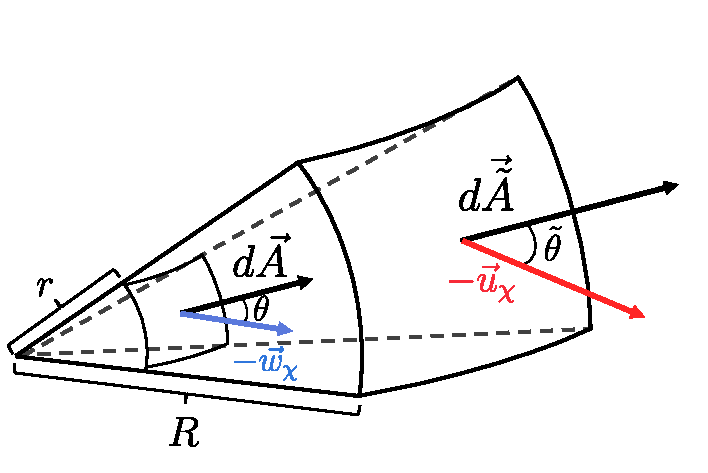
\includegraphics{img/chapter_3/capture_geometry.pdf}
    \caption{Geometry of the capture process. The azimuthal angles are not shown for simplicity as they can be integrated over trivially.}
    \label{fig:capturegeometry}
\end{figure}

The probability that the DM interacts with the constituents of the shell depends on the interaction rate, $\Omega(w_\chi)$, multiplied by the time spent in the shell, $dt = dr/\dot r$. Hence, the probability of scattering within the shell is
\begin{equation}
    \Omega(w_\chi) \frac{dr}{\dot r} = 2  \Omega(w_\chi)\frac{1}{w_\chi}\left(1 - \left(\frac{J_\chi}{r w_\chi}\right)^2 \right)^{-1/2} \Theta(J_{\mathrm{max}} - J_\chi)\,dr,\label{eq:int_prob_1}
\end{equation}
where the factor of 2 is due to the DM having two opportunities to pass through the shell, once when incoming and another after turning around\footnote{The radial velocity $\dot r$ is a standard result in orbital mechanics and can be obtained from the central force Lagrangian.}. The step-function is put in to ensure the angular momentum does not exceed its maximum allowed value. 

For a scattered DM to be considered captured, it must lose enough energy in the collision to become gravitationally bound. The rate at which a DM particle scatters from an initial velocity $w_\chi$ to a final velocity $v<v_e(r)$ is given by~\cite{Gould:1987ju_WeaklyInteractingMassive, Gould:1987ir_ResonantEnhancementsWIMP, Busoni:2017mhe_oct_Evaporationscatteringmomentum}
\begin{align}
    \Omega^{-}(w_\chi) &= \int_0^{v_e} R^-(w_\chi \rightarrow v) dv,\label{eq:down_rate_1}\\
    R^-(w_\chi \rightarrow v) & = \int n_T(r) \frac{d\sigma_{\chi T}}{dv} |\vec{w}_\chi -\vec{u}_T| f_T(u_T) \,d^3\vec{u}_T, \label{eq:diff_int_NR_gen}
\end{align}
with $R^-(w_\chi \rightarrow v)$ being the differential interaction rate, $n_T$ is the target number density, $u_T$ is the target velocity and $f_T(u_T)$ is the corresponding distribution function, and $d\sigma_{\chi T}/dv$ is the differential cross-section. The minus superscript is used to signify that this is the down scattering rate, i.e. the rate of interactions leading to the DM losing energy. 

Finally, we obtain the capture rate by multiplying Eqs.~\ref{eq:shell_flux} and~\ref{eq:int_prob_1} and integrate over the angular momentum to give the result
\begin{equation}
    C =\int_0^{R_\star} \,dr\, 4\pi r^2 \int_0^\infty\,du_\chi\, \frac{\rho_\chi}{m_\chi} \frac{\fMB(u_\chi)}{u_\chi} w_\chi(r)\Omega^-(w_\chi).
\end{equation}
This result is rather generic, as the choice of DM model will only dictate the form of the differential cross section in  Eq.~\ref{eq:diff_int_NR_gen}. In fact, as written above, the distribution function for the relative velocity far from the star can be any isotropic distribution function. The MB form was chosen as it allows for a simple analytic form. 

% To give a simple example, we neglect the thermal motion of the constituents, reducing the rate to
% \begin{align}
%     R^-(w_\chi \rightarrow v) = \frac{4 \mu_+^2}{\mu} n_T \frac{v}{w_\chi} \frac{d\sigma_{\chi T}}{d\cos\theta_{\mathrm{CM}}} \Theta\left(v - w\frac{|\mu_-|}{\mu_+}\right).
% \end{align}
% where $n_T$ is the local number density of the targets, and we have introduced the useful quantities $\mu$, $\mu_\pm$ that are
% \begin{equation}
%     \mu = \frac{m_\chi}{m_T}, \quad  \mu_\pm = \frac{\mu \pm 1}{2}.
% \end{equation}
% For the case of constant DM-target cross-section, we can compute the integral in Eq.~\ref{eq:down_rate_1}
% \begin{align}
%     R^-(w_\chi \rightarrow v) &= \frac{4 \mu_+^2}{\mu} n_T \frac{v}{w_\chi}\frac{\sigma_{\chi T}}{2} \Theta\left(v - w\frac{|\mu_-|}{\mu_+}\right),\\
%     \Omega^-(w_\chi) & = \frac{2\mu_+^2}{\mu} \frac{n_T \sigma_{\chi T}}{w_\chi} \left(v_e^2 - \frac{\mu_-^2}{\mu_+^2}w_\chi^2\right)\Theta\left(v_e^2 - \frac{\mu_-^2}{\mu_+^2}w_\chi^2\right).
% \end{align}

% It may be the case that the DM does not lose enough energy in a single scatter to become gravitationally bound to the star. If so, the capture probability must be modified for multi-scatter capture. \commMV{Gould and Bramante...}

%%%%%%%%%%%%%%%%%%%%%%%%%%%%%%%%%%%%%
%%%%%%%%%%%%%%%%%%%%%%%%%%%%%%%%%%%%%
%%%%%%%%%%%%%%%%%%%%%%%%%%%%%%%%%%%%%
\section{Capture in Compact Objects}
%%%%%%%%%%%%%%%%%%%%%%%%%%%%%%%%%%%%%
%%%%%%%%%%%%%%%%%%%%%%%%%%%%%%%%%%%%%
%%%%%%%%%%%%%%%%%%%%%%%%%%%%%%%%%%%%%

Having reviewed the capture process in non-relativistic stars, we can begin discussing the necessary modifications required when considering relativistic stars. In this section, we consider the two major modifications that need to be made: 
\begin{itemize}
    \item The corrections from General Relativity due to the extreme gravitational fields. This ultimately alters the flux of DM passing through the star, boosting it through gravitational focusing.
    \item Accounting for the relativistic and degenerate nature of the star's constituents in the interaction rate.
\end{itemize}

The former is generic to neutron stars and white dwarfs, while the latter is required for all NS constituents, but only the electrons in a WD are degenerate and relativistic. The ions of the WD are non-relativistic and non-degenerate and, hence, can be treated the same as the Sun's constituents. 

%%%%%%%%%%%%%%%%%%%%%%%%%%%%%%%%%%%%%
%%%%%%%%%%%%%%%%%%%%%%%%%%%%%%%%%%%%%
\subsection{General Relativistic Corrections to the Capture Rate}
%%%%%%%%%%%%%%%%%%%%%%%%%%%%%%%%%%%%%

Far from the star, the physics is the same as in the previous section. The deviations arise as the DM falls into he gravitational potential of the star. We begin by following the DM along its trajectory, moving from a distance $R\gg R_\star$ to a closer distance $r$. Hence, we are working in the DM rest frame and calculating the rate at which the DM passes through the shell \textit{per unit of proper time}, $\tau$. The proper time interval is related to the metric through
\begin{equation}
    d\tau^2 = B(r) dt^2 - A(r) dr^2 - r^2 d\Omega^2,
\end{equation}
with $B(r)$ and $A(r)$ defined in Chapter~\ref{chapter:compactobjects}. 

Following the same arguments as in the non-relativistic case, the flux of DM passing through the shell is 
\begin{equation}
    \frac{d N_\chi}{d\tau} = 2\pi \frac{\rho_\chi}{m_\chi}\frac{\fMB(u_\chi)}{u_\chi}\,du_\chi\,\frac{J_\chi \, dJ_\chi}{m_\chi^2},
\end{equation}
which takes the same form as Eq.~\ref{eq:shell_flux}, with the physical difference being that this is the rate with respect to the proper time.

The probability that DM scatters within the shell and is captured is $2\hat{\Omega}^-(r) d\tau$,
where $\hat{\Omega}^-(r)$ is the interaction rate with respect to the proper time, and $d\tau$ is the proper time taken to move from coordinate $r$ to $r + dr$. The factor of 2 once again accounts for the DM crossing the shell twice per orbit. For calculation purposes, we need to relate this to the interaction rate seen by a distant observer, $\Omega^-(r)$, that is done through
\begin{equation}
    \hat{\Omega}^-(r) d\tau = \frac{1}{\sqrt{g_{tt}}}\Omega^-(r)d\tau= \frac{1}{\sqrt{B(r)}}\Omega^-(r)d\tau.
\end{equation}
Now, the proper time that the DM spends inside a shell of thickness $dr$ will be\footnote{See Appendix~\ref{appendix:kin_heating} for the derivation of $\dot r = \frac{dr}{dt}$.}
\begin{equation}
    d\tau = \left( \frac{d\tau}{dt}\right) dt = B(r) \frac{dr}{\dot r} = \frac{\sqrt{B(r)} dr}{\sqrt{\frac{1}{A(r)} \left[ 1 - B(r)\left( 1 + \frac{J_\chi^2}{m_\chi^2 r^2} \right) \right]}}.
\end{equation}

Combining everything together gives us the differential capture rate, 
\begin{equation}
    dC =  2\pi  \frac{\rho_\chi}{m_\chi}\frac{\fMB(u_\chi)}{u_\chi}\,du_\chi\,\frac{dJ^2_\chi}{m_\chi^2} \frac{\Omega^-(r)\sqrt{A(r)} \,dr}{\sqrt{1 - B(r)\left( 1 + \frac{J_\chi^2}{m_\chi^2 r^2} \right)}}.
\end{equation}
As the total number of targets in the star, $N_T$, needs to satisfy
\begin{equation}
    N_T = \int_0^{R_\star} 4\pi r^2 n_T(r)\sqrt{A(r)}\,dr,
\end{equation}
where $n_T(r)$ is the number density that appears in the interaction rate, we absorb the factor $\sqrt{A(r)}$ into the definition of $n_T(r)$, such that $\Omega^-(r)\sqrt{A(r)}\rightarrow \Omega^-(r)$. This is due to the number densities obtained by solving the TOV equations already account for the $\sqrt{A(r)}$ factor. 

As before, we have $w_\chi^2(r) = u_\chi^2 + v_e^2(r)$, however as the escape velocity will be significantly larger than the ambient DM velocity far from the star, we can safely approximate $w_\chi^2(r)\approx v_e^2(r)$. 
In the relativistic case, the escape velocity can be defined as
\begin{equation}
    v_e^2(r) = \left(\frac{dl}{d\tau}\right)^2 = A(r) \left(\frac{dr}{d\tau}\right)^2 + r^2 \left(\frac{d\phi}{d\tau}\right)^2 = 1 - B(r),
\end{equation}
where $dl$ is a length element. 
The large boost from the escape velocity also removes the $u_\chi$ dependence in the kinematics of the interactions and allows us to perform the integration over the initial DM velocity, yielding an overall factor of
\begin{equation}
    \int_0^\infty \frac{\fMB(u_\chi)}{u_\chi} du_\chi = \frac{1}{v_\star}\erf\left(\sqrt{\frac{3}{2}}\frac{v_\star}{v_d}\right).
\end{equation}

To integrate over $J^2_\chi$, we need the maximum angular momentum the DM can achieve as it passes through the shell. This can be obtained by requiring the argument of the radical above to remain positive, giving
\begin{equation}
    J_\mathrm{max} = \sqrt{\frac{1 - B(r)}{B(r)}} m_\chi r.
\end{equation}
The factor of $1/\sqrt{B}$ arises due to the gravitational focusing of the incoming flux of DM~\cite{Kouvaris:2007ay_WIMPAnnihilationCooling}.
% The angular momentum is given by
% \begin{equation}
%     J_\chi = m_\chi r^2\frac{d\phi}{d\tau}  \leq \frac{m_\chi}{\sqrt{B(r)}} r w_\chi(r) = J_\mathrm{max},
% \end{equation}
% This can be obtained by requiring that the contents of the square root above remain positive, giving
% \begin{equation}
%     J_\mathrm{max}^2 = \frac{1-B(r)}{B(r)} m_\chi^2 r^2,
% \end{equation}

Putting everything together, and integrating over the radius of the star, we are left with the final result for the capture rate of
\begin{equation}
    C =\frac{4\pi}{v_\star}\frac{\rho_\chi}{m_\chi} \erf\left(\sqrt{\frac{3}{2}}\frac{v_\star}{v_d}\right) \int_0^{R_\star}  r^2\frac{\sqrt{1 - B(r)}}{B(r)}\Omega^-(r)\,dr.
\end{equation}

%%%%%%%%%%%%%%%%%%%%%%%%%%%%%%%%%%%%%
%%%%%%%%%%%%%%%%%%%%%%%%%%%%%%%%%%%%%
\subsection{Interaction Rate for Degenerate Targets}
%%%%%%%%%%%%%%%%%%%%%%%%%%%%%%%%%%%%%
%%%%%%%%%%%%%%%%%%%%%%%%%%%%%%%%%%%%%

%%%%%%%%%%%%%%%%%%%%%%%%%%%%%%%%%%%%%
%%%%%%%%%%%%%%%%%%%%%%%%%%%%%%%%%%%%%
%%%%%%%%%%%%%%%%%%%%%%%%%%%%%%%%%%%%%
\section{White Dwarfs: Electron Targets}
%%%%%%%%%%%%%%%%%%%%%%%%%%%%%%%%%%%%%
%%%%%%%%%%%%%%%%%%%%%%%%%%%%%%%%%%%%%
%%%%%%%%%%%%%%%%%%%%%%%%%%%%%%%%%%%%%

%%%%%%%%%%%%%%%%%%%%%%%%%%%%%%%%%%%%%
%%%%%%%%%%%%%%%%%%%%%%%%%%%%%%%%%%%%%
%%%%%%%%%%%%%%%%%%%%%%%%%%%%%%%%%%%%%
\section{Neutron Stars: Leptoinc Targets}
%%%%%%%%%%%%%%%%%%%%%%%%%%%%%%%%%%%%%
%%%%%%%%%%%%%%%%%%%%%%%%%%%%%%%%%%%%%
%%%%%%%%%%%%%%%%%%%%%%%%%%%%%%%%%%%%%
